\documentclass[aspectratio=169,10pt]{beamer}

% ── Theme & Colors ──────────────────────────────────────
\usetheme{Madrid}
\usecolortheme{whale}

\definecolor{kfupm}{RGB}{0,84,60}
\definecolor{accent}{RGB}{0,150,136}
\definecolor{darkbg}{RGB}{33,37,41}
\definecolor{lightgray}{RGB}{245,245,245}
\definecolor{codebg}{RGB}{240,240,240}

\setbeamercolor{structure}{fg=kfupm}
\setbeamercolor{palette primary}{bg=kfupm,fg=white}
\setbeamercolor{palette secondary}{bg=accent,fg=white}
\setbeamercolor{palette tertiary}{bg=darkbg,fg=white}
\setbeamercolor{frametitle}{bg=kfupm,fg=white}
\setbeamercolor{title}{bg=kfupm,fg=white}
\setbeamercolor{block title}{bg=kfupm,fg=white}
\setbeamercolor{block body}{bg=lightgray,fg=darkbg}
\setbeamercolor{block title alerted}{bg=red!80!black,fg=white}
\setbeamercolor{block body alerted}{bg=red!5,fg=darkbg}
\setbeamercolor{block title example}{bg=accent,fg=white}
\setbeamercolor{block body example}{bg=accent!5,fg=darkbg}
\setbeamercolor{item}{fg=kfupm}

\setbeamerfont{title}{size=\Large,series=\bfseries}
\setbeamerfont{frametitle}{size=\large,series=\bfseries}
\setbeamerfont{framesubtitle}{size=\small}
\setbeamertemplate{blocks}[rounded][shadow=false]

% ── Packages ────────────────────────────────────────────
\usepackage[T1]{fontenc}
\usepackage[utf8]{inputenc}
\usepackage{lmodern}
\usepackage{graphicx}
\usepackage{booktabs}
\usepackage{tabularx}
\usepackage{listings}
\usepackage{tikz}
\usetikzlibrary{positioning}
\usepackage{pifont}
\newcommand{\ico}[1]{\textcolor{kfupm}{\ding{#1}}}
\usepackage{hyperref}

\newcolumntype{Y}{>{\raggedright\arraybackslash}X}

\lstdefinestyle{slidecode}{
  basicstyle=\ttfamily\scriptsize,
  backgroundcolor=\color{codebg},
  frame=single,
  breaklines=true,
  columns=fullflexible,
  keepspaces=true
}

% ── Metadata ────────────────────────────────────────────
\title[DVSA Remediation]{DVSA Vulnerability Discovery \& Remediation}
\subtitle[ICS-344]{ICS-344 --- Information Security}
\author[Husain, Ali, Abdulwahed]{Husain Al Muallim \and Ali Al Qatari \and Abdulwahed Zuhair Adi}
\institute{King Fahd University of Petroleum and Minerals}
\date[May 2026]{Term 252 --- May 2026}

% ── Slide counter ───────────────────────────────────────
\setbeamertemplate{navigation symbols}{}
\setbeamertemplate{footline}{
  \leavevmode\hbox{%
    \begin{beamercolorbox}[wd=.333\paperwidth,ht=2.5ex,dp=1ex,center]{palette primary}
      \usebeamerfont{author in head/foot}\insertshortauthor
    \end{beamercolorbox}%
    \begin{beamercolorbox}[wd=.334\paperwidth,ht=2.5ex,dp=1ex,center]{palette secondary}
      \usebeamerfont{title in head/foot}\insertshorttitle
    \end{beamercolorbox}%
    \begin{beamercolorbox}[wd=.333\paperwidth,ht=2.5ex,dp=1ex,right]{palette tertiary}
      \usebeamerfont{date in head/foot}\insertframenumber{}/\inserttotalframenumber\hspace*{2ex}
    \end{beamercolorbox}%
  }%
}

% ── Lesson slide helper ─────────────────────────────────
% #1=number, #2=title, #3=vuln type, #4=component, #5=root cause, #6=exploit summary, #7=fix summary, #8=lesson learned
\newcommand{\lessonslide}[8]{
\begin{frame}{Lesson #1: #2}
\begin{columns}[T]
\begin{column}{0.48\textwidth}
  \begin{alertblock}{\ding{72} Vulnerability}
    \textbf{Type:} #3\\
    \textbf{Component:} \texttt{#4}
  \end{alertblock}
  \begin{block}{\ding{46} Root Cause}
    #5
  \end{block}
\end{column}
\begin{column}{0.48\textwidth}
  \begin{alertblock}{\ding{55} Exploit}
    #6
  \end{alertblock}
  \begin{exampleblock}{\ding{51} Fix \& Verification}
    #7
  \end{exampleblock}
\end{column}
\end{columns}
\vspace{0.3em}
\centering\small\textcolor{kfupm}{\ding{228}~\textbf{Takeaway:} #8}
\end{frame}
}

\begin{document}

% ════════════════════════════════════════════════════════
%   TITLE SLIDE
% ════════════════════════════════════════════════════════
{
\begin{frame}[plain,noframenumbering]
\begin{tikzpicture}[remember picture,overlay]
  \fill[kfupm] (current page.south west) rectangle (current page.north east);
  \node[anchor=center] at (current page.center) {
    \begin{minipage}{0.86\textwidth}
      \centering\color{white}
      {\Large\bfseries King Fahd University of Petroleum and Minerals\par}
      \vspace{0.35cm}
      \rule{0.62\textwidth}{0.4pt}\par
      \vspace{0.55cm}
      {\fontsize{24}{30}\selectfont\bfseries DVSA Vulnerability Discovery\\[2pt]\& Remediation\par}
      \vspace{0.45cm}
      {\large ICS-344 --- Information Security\par}
      \vspace{0.15cm}
      {\normalsize Term 252 \quad\textbullet\quad Team 2 \quad\textbullet\quad Sections 1 \& 2\par}
      \vspace{0.65cm}
      \rule{0.50\textwidth}{0.4pt}\par
      \vspace{0.45cm}
      {\normalsize Husain Al Muallim \quad\textbullet\quad Ali Al Qatari \quad\textbullet\quad Abdulwahed Zuhair Adi\par}
      \vspace{0.15cm}
      {\small 202163730 \quad\textbullet\quad 202279780 \quad\textbullet\quad 202256380\par}
      \vspace{0.45cm}
      {\small May 2026\par}
    \end{minipage}
  };
\end{tikzpicture}
\end{frame}
}

% ════════════════════════════════════════════════════════
%   AGENDA
% ════════════════════════════════════════════════════════
\begin{frame}{Agenda}
\tableofcontents
\end{frame}

% ════════════════════════════════════════════════════════
\section{Project Overview}
% ════════════════════════════════════════════════════════

\begin{frame}{Project Scope \& Deployment}
\begin{columns}[T]
\begin{column}{0.52\textwidth}
  \begin{block}{\ding{68} Scope}
    \begin{itemize}
      \item Deploy OWASP DVSA in a non-production AWS account
      \item Exploit \textbf{10 official vulnerability lessons}
      \item Apply remediations and verify each fix
      \item Document with structured 10-part analysis
    \end{itemize}
  \end{block}
\end{column}
\begin{column}{0.44\textwidth}
  \begin{block}{\ding{70} Deployment}
    \begin{itemize}
      \item \textbf{Region:} us-east-1
      \item \textbf{Stack:} serverlessrepo-OWASP-DVSA
      \item \textbf{Services:} S3, API Gateway, Lambda, DynamoDB, SQS, Cognito, IAM, SES, CloudWatch, CloudTrail
    \end{itemize}
  \end{block}
\end{column}
\end{columns}
\end{frame}

\begin{frame}{Architecture \& Request Pipeline}
\begin{center}
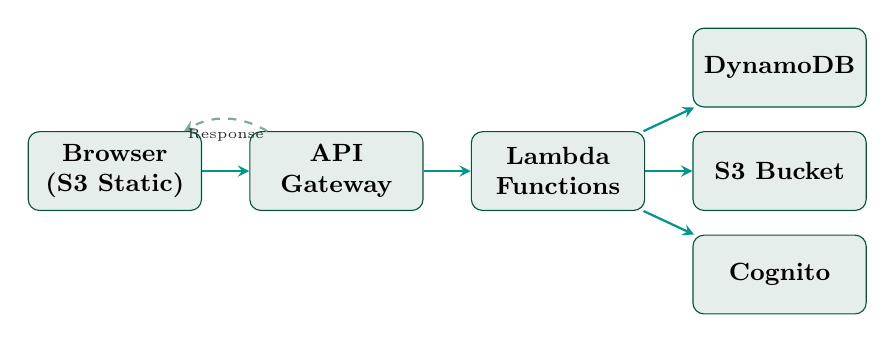
\begin{tikzpicture}[
  box/.style={draw=kfupm, fill=kfupm!10, rounded corners=4pt, minimum height=1cm, minimum width=2.2cm, align=center, font=\small\bfseries},
  arr/.style={->, thick, color=accent, >=stealth},
  node distance=0.6cm
]
  \node[box] (browser) {Browser\\(S3 Static)};
  \node[box, right=of browser] (apigw) {API\\Gateway};
  \node[box, right=of apigw] (lambda) {Lambda\\Functions};
  \node[box, above right=0.3cm and 0.6cm of lambda] (dynamo) {DynamoDB};
  \node[box, right=0.6cm of lambda] (s3) {S3 Bucket};
  \node[box, below right=0.3cm and 0.6cm of lambda] (cognito) {Cognito};
  
  \draw[arr] (browser) -- (apigw);
  \draw[arr] (apigw) -- (lambda);
  \draw[arr] (lambda) -- (dynamo);
  \draw[arr] (lambda) -- (s3);
  \draw[arr] (lambda) -- (cognito);
  \draw[arr, dashed, color=kfupm!50] (apigw) to[bend right=30] node[below, font=\tiny, color=darkbg] {Response} (browser);
\end{tikzpicture}
\end{center}
\vspace{0.3em}
\begin{block}{\ding{220} Pipeline}
  Browser $\rightarrow$ API Gateway $\rightarrow$ Lambda (e.g., \texttt{ORDER-MANAGER}) $\rightarrow$ DynamoDB / S3 / Cognito $\rightarrow$ Response
\end{block}
\end{frame}

\begin{frame}{Methodology \& Tools}
\begin{columns}[T]
\begin{column}{0.48\textwidth}
  \begin{block}{\ding{46} Tools Used}
    \begin{itemize}
      \item \texttt{curl}, \texttt{jq}, Python \texttt{requests}
      \item Browser DevTools (Network, Console)
      \item AWS Console (Lambda, IAM, S3, API GW)
      \item AWS CLI, IAM Policy Simulator
      \item CloudWatch Logs, CloudTrail
    \end{itemize}
  \end{block}
\end{column}
\begin{column}{0.48\textwidth}
  \begin{block}{\ding{51} Process}
    \begin{enumerate}
      \item Validate environment end-to-end
      \item Identify \& reproduce vulnerability
      \item Capture evidence (screenshots, logs)
      \item Apply targeted fix at root cause
      \item Re-run exploit to verify fix
      \item Confirm normal workflow intact
    \end{enumerate}
  \end{block}
\end{column}
\end{columns}
\end{frame}

% ════════════════════════════════════════════════════════
\section{Lessons 1--3: Injection, Auth, Data Exposure}
% ════════════════════════════════════════════════════════

\lessonslide{01}{Event Injection}
{Insecure Deserialization / RCE}
{DVSA-ORDER-MANAGER}
{\texttt{node-serialize.unserialize()} uses \texttt{eval()} internally, executing attacker-controlled code from request body.}
{Crafted JSON with \texttt{\_\$\$ND\_FUNC\$\$\_} tag executed arbitrary JS on Lambda, writing/reading files in \texttt{/tmp}.}
{Replaced \texttt{unserialize()} with \texttt{JSON.parse()}. Post-fix: same payload no longer executes; CloudWatch clean.}
{Never use libraries that evaluate user input as code. Use strict, safe parsers for all untrusted data.}

\lessonslide{02}{Broken Authentication}
{Missing API Gateway Authorizer}
{DVSA-ORDER-MANAGER}
{API Gateway \texttt{/order} POST had no Cognito Authorizer. Any JWT---valid or forged---was forwarded to Lambda.}
{Regular user called \texttt{admin-orders} action and received all users' order data without admin privileges.}
{Attached Cognito Authorizer to API Gateway + added \texttt{is\_admin} check in Lambda. Post-fix: returns 401/403.}
{Enforce auth at the edge (API Gateway) \emph{and} in code. Defense in depth prevents single-layer failures.}

\lessonslide{03}{Sensitive Data Exposure}
{Missing Authorization in Lambda}
{DVSA-ADMIN-GET-RECEIPT}
{Lambda had zero auth checks. Any caller could invoke it directly and receive a signed S3 URL for all receipts.}
{Invoked Lambda via Console test with arbitrary date params; received signed URL to download all customer receipts.}
{Added \texttt{requestContext} check + admin ARN verification. Post-fix: returns ``Access denied'' (1.6ms vs 4.3s).}
{``Admin'' in the name doesn't enforce access. Lambda functions can bypass API Gateway; auth must be in-function.}

% ════════════════════════════════════════════════════════
\section{Lessons 4--6: Cloud Config, Access Control, DoS}
% ════════════════════════════════════════════════════════

\lessonslide{04}{Insecure Cloud Configuration}
{Open S3 Bucket}
{dvsa-receipts-bucket}
{S3 bucket deployed without ``Block Public Access.'' Broad IAM policies allowed external principals to write objects.}
{Used \texttt{aws s3 cp} with a ``hacker'' profile to upload arbitrary files into the receipts bucket successfully.}
{Enabled \textbf{Block All Public Access} on S3 bucket. Post-fix: upload returns Access Denied; receipts still work.}
{Always enable Block Public Access unless explicitly justified. Default-open CloudFormation configs cause breaches.}

\lessonslide{05}{Broken Access Control}
{IDOR --- No Ownership Check}
{DVSA-ORDER-MANAGER}
{Lambda extracted \texttt{order-id} from body without verifying the JWT user owns that order in DynamoDB.}
{User B sent \texttt{curl} with User C's order ID and received C's full order details (address, items, payment).}
{Added \texttt{userOwnsOrder()} check before dispatching. Post-fix: returns ``could not find order'' for non-owners.}
{APIs must enforce resource ownership server-side. Front-end restrictions alone are trivially bypassed.}

\lessonslide{06}{Denial of Service}
{No Rate Limiting on API Gateway}
{DVSA-PAYMENT-PROCESSOR}
{No throttling on API Gateway; account had only 10 concurrent Lambda slots. Easily saturated by parallel requests.}
{Python threading script sent 15+ parallel billing requests; legitimate users got connection resets and 500 errors.}
{Enabled API Gateway stage throttling (Rate=10/s, Burst=2). Post-fix: excess requests rejected at gateway layer.}
{Availability is a security property. Serverless concurrency is finite---rate-limit critical endpoints like billing.}

% ════════════════════════════════════════════════════════
\section{Lessons 7--10: Privilege, Logic, Deps, Exceptions}
% ════════════════════════════════════════════════════════

\lessonslide{07}{Over-Privileged Function}
{Excessive IAM Permissions}
{SendReceiptFunctionRole}
{Role had \texttt{AmazonSESFullAccess} + full S3 + full DynamoDB. A compromised Lambda would inherit all capabilities.}
{Policy Simulator confirmed: \texttt{s3:PutObject}, \texttt{dynamodb:Scan}, all SES actions were \textbf{allowed}.}
{Replaced 3 broad policies with 1 scoped inline policy (S3 GetObject + SES SendEmail only). Simulator: denied.}
{Apply least privilege always. Use CloudTrail Generate Policy to right-size permissions based on actual usage.}

\lessonslide{08}{Logic Vulnerabilities}
{Race Condition in Order Update}
{DVSA-ORDER-UPDATE}
{Status check used \texttt{> 110} instead of \texttt{> 100}, allowing modification during billing window (status 100).}
{Paid for cheap items, then updated order to expensive items before status advanced past 100. ``Cart updated'' returned.}
{Changed threshold to \texttt{> 100}. Post-fix: updates on non-open orders return ``order already paid or in progress.''}
{Logic flaws evade scanners. State-machine transitions must be strict; review boundary conditions carefully.}

\lessonslide{09}{Vulnerable Dependencies}
{Known CVE in node-serialize}
{DVSA-ORDER-MANAGER}
{\texttt{package.json} included \texttt{node-serialize} v0.0.4---CVE-2017-5941, CVSS 9.8 Critical (RCE via \texttt{eval}).}
{NVD lookup confirmed critical severity. The package was actively used for deserialization (see Lesson 01).}
{Removed \texttt{node-serialize} from \texttt{package.json}; code already uses \texttt{JSON.parse()}. Lambda deploys cleanly.}
{Audit dependencies regularly (\texttt{npm audit}, Snyk). A single vulnerable package can compromise everything.}

\lessonslide{10}{Unhandled Exceptions}
{Stack Trace Leakage}
{DVSA-ORDER-GET}
{Missing try/except: a malformed request raised \texttt{KeyError}, returning full traceback with file paths to client.}
{Sent \texttt{\{"action":"get"\}} without \texttt{order-id}; response contained \texttt{/var/task/get\_order.py} and line numbers.}
{Wrapped handler in try/except with \texttt{safe\_error()} returning generic messages. Internals logged server-side only.}
{Never expose stack traces to clients. Catch all exceptions at the handler boundary and return sanitized errors.}

% ════════════════════════════════════════════════════════
\section{Key Takeaways}
% ════════════════════════════════════════════════════════

\begin{frame}{Security Themes Across All Lessons}
\begin{columns}[T]
\begin{column}{0.48\textwidth}
  \begin{block}{\ding{70} Defense in Depth}
    Security at multiple layers: API Gateway auth, Lambda code validation, IAM policies, and cloud resource config.
  \end{block}
  \vspace{0.3em}
  \begin{block}{\ding{49} Least Privilege}
    IAM roles scoped to exact actions needed. Over-privileged roles amplify the blast radius of any compromise.
  \end{block}
  \vspace{0.3em}
  \begin{block}{\ding{46} Input Validation}
    All user input is untrusted. Use safe parsers, validate schemas, and never evaluate input as code.
  \end{block}
\end{column}
\begin{column}{0.48\textwidth}
  \begin{block}{\ding{68} Dependency Hygiene}
    Regularly audit packages for CVEs. Remove unused libraries. Minimize attack surface.
  \end{block}
  \vspace{0.3em}
  \begin{block}{\ding{72} Safe Error Handling}
    Never expose internals to clients. Log verbose details server-side; respond with generic messages.
  \end{block}
  \vspace{0.3em}
  \begin{block}{\ding{220} Availability Controls}
    Rate limiting and throttling protect shared serverless resources from exhaustion attacks.
  \end{block}
\end{column}
\end{columns}
\end{frame}

\begin{frame}{Vulnerability Summary Matrix}
\centering
\footnotesize
\begin{tabularx}{\textwidth}{c >{\raggedright}p{2.3cm} >{\raggedright}p{3cm} >{\raggedright}p{2.8cm} >{\raggedright\arraybackslash}p{3.5cm}}
\toprule
\textbf{\#} & \textbf{Lesson} & \textbf{Vulnerability} & \textbf{Component} & \textbf{Fix} \\
\midrule
01 & Event Injection & Insecure deserialization & ORDER-MANAGER & Replace with JSON.parse() \\
02 & Broken Auth & Missing authorizer & API Gateway & Attach Cognito Authorizer \\
03 & Data Exposure & No auth in Lambda & ADMIN-GET-RECEIPT & Add requestContext + ARN check \\
04 & Cloud Config & Open S3 bucket & Receipts bucket & Block All Public Access \\
05 & Access Control & IDOR / no ownership & ORDER-MANAGER & userOwnsOrder() check \\
06 & DoS & No rate limiting & API Gateway & Stage-level throttling \\
07 & Over-Privilege & Excessive IAM & SendReceipt role & Scoped inline policy \\
08 & Logic Flaw & Race condition & ORDER-UPDATE & Status threshold $>$100 \\
09 & Vuln Deps & CVE-2017-5941 & package.json & Remove node-serialize \\
10 & Exceptions & Stack trace leak & ORDER-GET & try/except + safe\_error() \\
\bottomrule
\end{tabularx}
\end{frame}

% ════════════════════════════════════════════════════════
%   CLOSING
% ════════════════════════════════════════════════════════
{
\begin{frame}[plain,noframenumbering]
\begin{tikzpicture}[remember picture,overlay]
  \fill[kfupm] (current page.south west) rectangle (current page.north east);
  \node[anchor=center] at (current page.center) {
    \begin{minipage}{0.82\textwidth}
      \centering\color{white}
      {\fontsize{28}{34}\selectfont\bfseries Thank You\par}
      % \vspace{0.7cm}
      % {\Large Questions?\par}
      % \vspace{1.0cm}
      \rule{0.52\textwidth}{0.4pt}\par
      \vspace{0.45cm}
      {\normalsize Husain Al Muallim \quad\textbullet\quad Ali Al Qatari \quad\textbullet\quad Abdulwahed Zuhair Adi\par}
      \vspace{0.35cm}
      {\small ICS-344 --- Term 252 --- Team 2\par}
    \end{minipage}
  };
\end{tikzpicture}
\end{frame}
}

\end{document}
